\subsection{Deduplication ratio} \label{sec:dedup_ratio}

%\subsection{Overview of file duplicates} \paragraph{File repeat count}

%The first step of our deduplication analysis is to calculate the file repeat
%count based on the file digests. Then we calculated the deduplication ratio
%using the savings after elimiation of file duplicates in terms of file count
%and capacity.

In Docker registry, layers are shared among different images to eliminate
duplicates.  In this section, we investigate if layer-level content addressable
is enough for Docker registry to mitigate redundancy.  Specifically, we look in
to the sharing rate of layers across images to calculate how much space is
saved by using layer-level content addressable storage.  We also investigate
that how much redundant data exists across images.

\paragraph{Layer reference count \& current deduplication ratio}

\begin{figure}
	\centering
	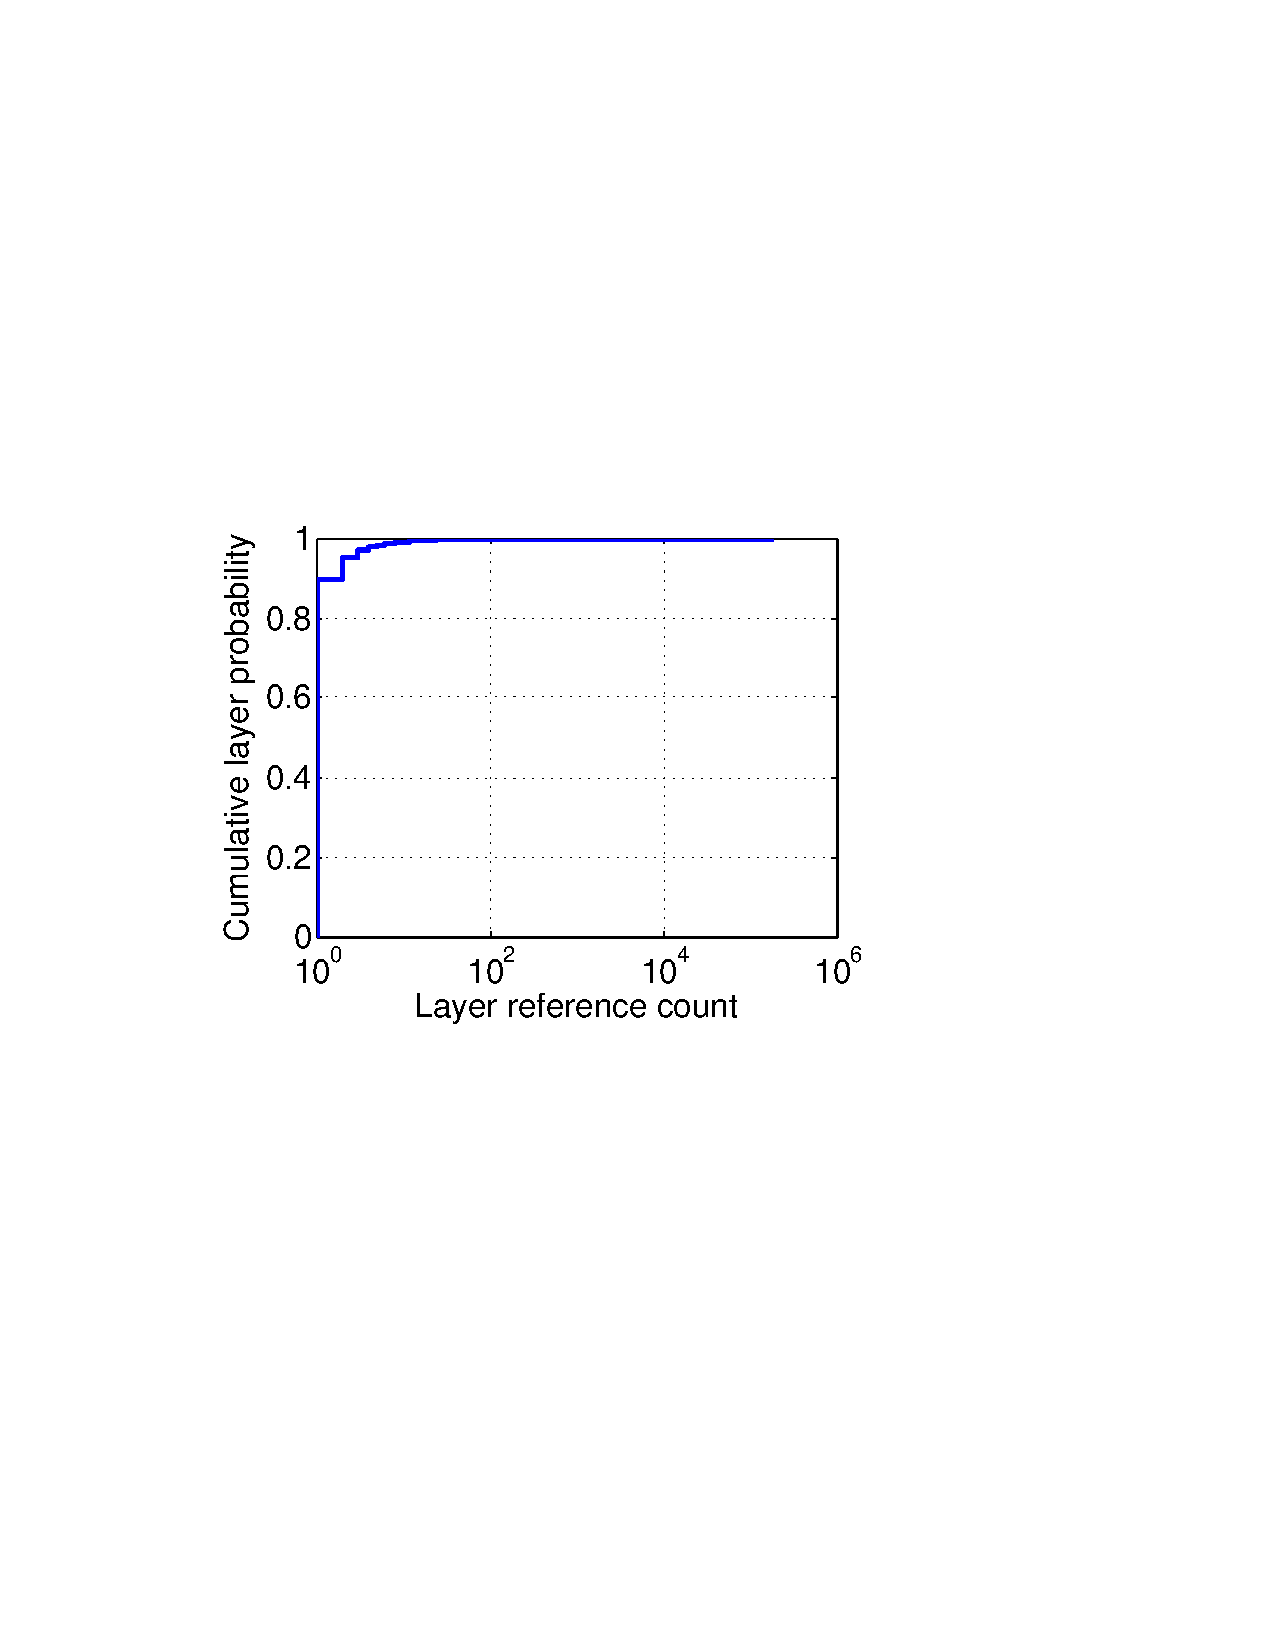
\includegraphics[width=0.21\textwidth]{graphs/shared-cnt-cdf.pdf}
	\caption{CDF of layer reference count.
	}
	\label{fig:ref_count}
\end{figure}


We analyzed all image manifests and count for each layer, how many times it is
referenced by an image.
%
Figure~\ref{fig:ref_count} shows that around 90\% of layers are only reference
by a single image while 95\% are reference by not more than 2 images.
%
Similarly, 99\% of layers are shared among less than 25 images. 
%
Accordingly, we calculated the total storage space consumed before layer-level
content addressability was adopted, which was 84.75 TB.  Thus the redundant
ratio achieved by layer-level content addressability is around 1.8.
%Figure~\ref{} shows the absolute values, revealing that almost 1.5 million
%images are only referenced once.  \acomment{Figure is missing} While there is
%again a large spectrum of reference counts, the maximum is 33,428, the vast
%majority of layers is not shared. 
%
This hints that the layer-based approach to improve storage efficiency is
barely utilized and there is room for improvement in how to construct more
sharable layers.
%
\emph{These findings reveal that layer level content addressable store has not
been very successful and most of the layers that exists in Docker Hub are not
shared among images.
	%
	Hence, there is a dire need of a better redundancy management.}

\paragraph{File repeat count}
%\paragraph{Full file duplicates}
\begin{figure} \centering
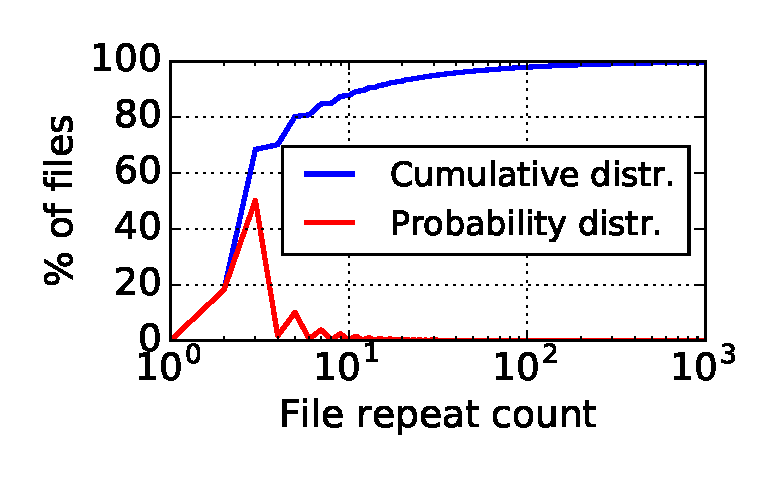
\includegraphics[width=0.45\textwidth]{graphs/File_repeat_count.eps}
\caption{File repeat count distribution.  } \label{fig:file-repeat-cnt}
\end{figure}

Figure~\ref{fig:file-repeat-cnt} shows the cumulative and probability
distribution of file repeat count.  \textit{We see that majority of files have
more than one copies (99.42\%).  Most files have a small repeat count.} For
instance, almost 90\% of files have equal or less than 10 copies. Around 50\%
of files have 4 copies. The file that has the maximum repeat count is an empty
file, which means that many users create and store empty files in their images.

\paragraph{Deduplication ratio}
%As discussed in compression ratio analysis, we see that there is redundant
%data in both layers and images.  We conducted simple form of deduplication to
%Interestingly,
Next, we calculate deduplication ratio in terms of file count and capacity for
the complete uncompressed dataset (Table~\ref{tbl:overall-redundant_ratio}).
%the redundant file overhead of the uncompressed dataset 
We find that majority of the files have more than one copy (99.42\%), which
take up over 89\% of capacity.  After elimination of file duplicates, the
percentage of such files decrease from 99.42\% to 2.59\%.  Overall, only 3.17\%
(23.92 TB) of files are unique files while 96.83\% of files (143.28 TB) are
redundant copies. Correspondingly, the deduplication ratio is 96.83\% and
85.69\% in terms of file count and capacity, respectively.
% Table~\ref{tbl:overall-redundant_ratio} summaries the overall redundant file
% overhead in terms of file count and capacity.

\textit{Finding 1: Majority of files in Docker registry are duplicates which
occupy most of capacity, indicating that Docker Hub has severe redundancy
problem.}

%\begin{figure} \centering \subfigure[Redundant file overhead in terms of file
%count]{\label{fig:over-dup-overhead-cnt} \includegraphics
%[width=0.21\textwidth]{graphs/dup-ratio-cnt.pdf} } \subfigure[Redundant file
%overhead in terms of capacity]{\label{fig:over-dup-overhead-cap}
%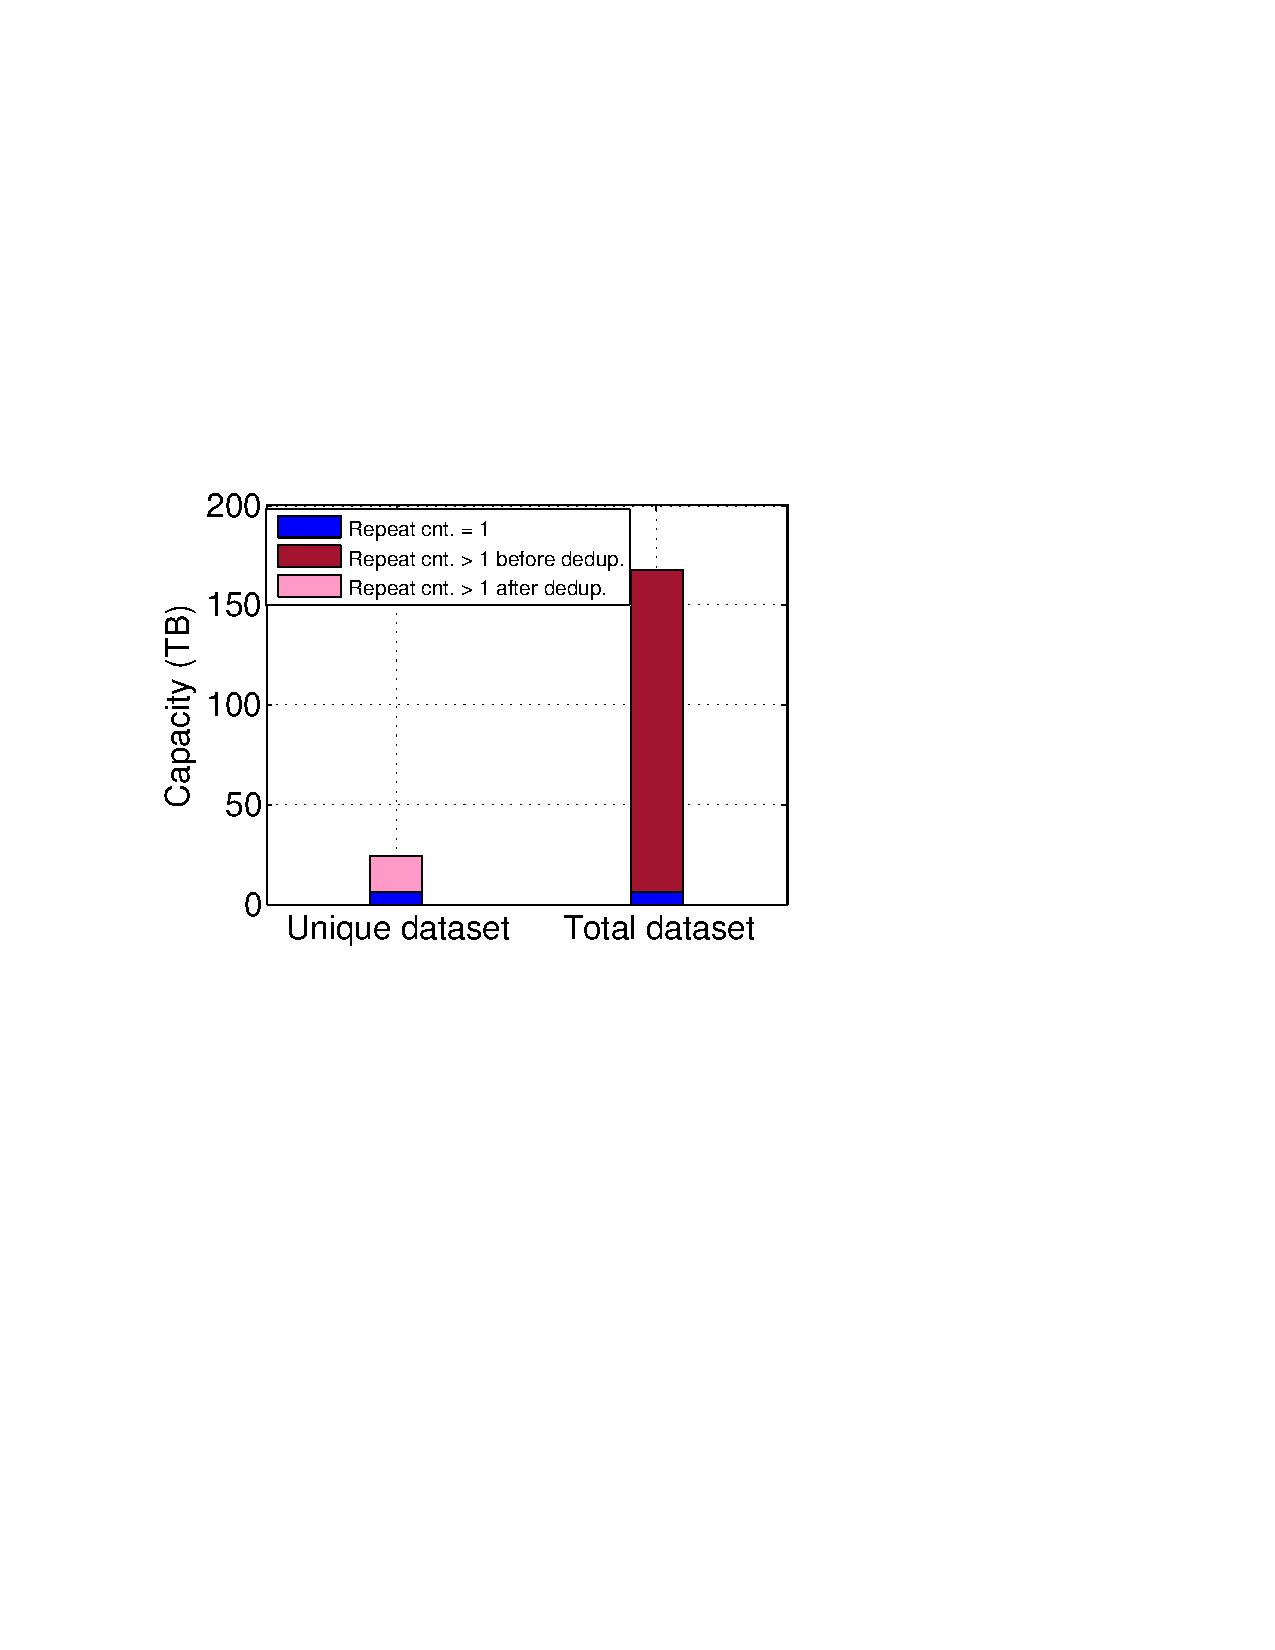
\includegraphics [width=0.225\textwidth]{graphs/dup-ratio-cap.pdf} }
%\caption{Redundant file overhead.} \label{fig:over-dup-overhead} \end{figure}

\begin{table} \centering \scriptsize  
	%\begin{minipage}{.5\linewidth}
	\caption{Redundant ratio in terms of file count and capacity}
\label{tbl:overall-redundant_ratio} \begin{tabular}{|l|l|l|}%p{0.14\textwidth}
\hline  & File count & Capacity \\ \hline Repeat cnt = 1 & 0.58\% & 10.87\%\\
\hline Repeat cnt $>$ 1 after dedup. & 2.59\% & 3.44\%\\ \hline Repeat cnt $>$
1 before dedup.  & 99.42\%  & 89.13\%\\ \hline Unique dataset (Uncompressed) &
3.17\% (167,251,437)  &  14.31\% (23.92 TB) \\ \hline Total dataset
(Uncompressed) & 5,278,465,130 & 167.20 TB \\ \hline 	
		%\hline 
	\end{tabular} \end{table} 

%\subsection{Cross image sharing}

%\paragraph{Cross layer sharing}
%
%%<<<<<<< HEAD \begin{figure} \centering \subfigure[CDF of cross-layer shared
%file ratio.]{\label{fig:layer-dedup-ratio} \includegraphics
%[width=0.22\textwidth]{graphs/layer-dup-ratio-cdf} } \subfigure[CDF of
%cross-image shared file ratio.]{\label{fig:image-dedup-ratio} \includegraphics
%[width=0.22\textwidth]{graphs/image-dup-ratio-pdf} } \caption{Cross layer
%sharing and cross image sharing} \label{fig:dedup-ratio} \end{figure} 
%
%Based on the high deduplication ratio, we guess that a large amount of files
%are shared between layers and the large potential from deduplication is due to
%files sharing between layers. Cross layer shared files are files that stored
%in more than one layers. There could be a high probability for Docker
%registry. For example, different developers work on same source codes and
%build same executables in their layers. Now, we calculated the percentage of
%cross layer shared files for each layer as shown in
%Figure~\ref{fig:layer-dedup-ratio}. 
% 
%%======= %Based on the high deduplication ratio, we infer that there is a
%great %potential of deduplication as large amount of files %are shared between
%the layers.  Cross layer shared files are files that are stored in more than
%one layers.  %There could be a high probability for Docker registry.  %For
%example, different developers work on same source codes and build same
%%executables in their layers.  % %>>>>>>>
%888904bc46b49ab605af4f202d35c8d68f7e868f %The analysis of compression ratio
%shows plenty redundant data exist in individual layers.  % %We define two
%duplicate ratio for layers: intra-layer duplicate ratio and inter-layer
%duplicate ratio. Intra-layer duplicate ratio $r_{intra\_ldedup.}$ is
%calculated as: %$r_{intra\_ldedup.} = \frac{S_{un.\_l} -
%S_{un.\_ldedup.}}{S_{un.\_l}}$, where $S_{un.\_l}$ is the uncompressed layer
%size while $S_{un.\_ldedup.}$ is the uncompressed layer size after removing
%the intra-layer duplicate files. Inter-layer duplicate ratio
%$r_{inter\_ldedup.}$ is calculated as: %$r_{inter\_ldedup.} = \frac{S_{un.\_l}
%- S_{un.\_sldedup.}}{S_{un.\_l}}$, where $S_{un.\_l}$ is the uncompressed
%layer size while $S_{un.\_sldedup.}$ is the uncompressed layer size after
%removing the inter-layer duplicate files.  %
%%Figure~\ref{fig:layer-dedup-ratio} shows the cross layer sharing file
%duplicate ratio %in terms of file count and capacity. %As shown in
%Figure~\ref{fig:layer-dedup-cdf}, %\nancomment{following description have
%problem.} %90\% of layers contains less than 53\% of intra-layer redundant
%files while %<<<<<<< HEAD 90\% of layers contains bigger than 97.6\% of files
%that are cross layer shared files. Similar to images, we also calculated the
%percentage of cross image shared files for each image as shown in
%Figure~\ref{fig:image-dedup-ratio}. 90\% of images contains bigger than 99.4\%
%of files that are cross image shared files, indicating that majority of files
%are replicated cross different images and cross layers.
%
%\textit{Finding 2: Majority duplicate files are stored cross layers and cross
%images, indicating developers store same files in containers as other
%developers.} %======= Figure~\ref{fig:layer-dedup-ratio} shows percentage of
%cross layer shared files for each layer. We find that 90\% of layers contain
%more than 97.6\% of files that are shared across layers. We also calculate the
%percentage of files that are shared across images. As shown in
%Figure~\ref{fig:layer-dedup-ratio}, 90\% of images contain more than 99.4\% of
%files that are shared across images, indicating that majority of files are
%replicated across different images and layers.
%
%\textit{Finding 2: Majority duplicate files are stored cross layers and cross
%images, indicating developers store same files in containers as other
%developers.} >>>>>>> 888904bc46b49ab605af4f202d35c8d68f7e868f \nancomment{one
%graph} Figure~\ref{fig:image-dedup-ratio} shows the intra/inter-image
%duplicate ratio in terms of file count and capacity.  90\% of images contains
%less than 54.4\% of intra-image redundant files while
%Figure~\ref{fig:layer-dedup_hist} shows that 0.2 M of images contains 0.45 of
%the intra-image duplicate files. We manually inspect few of these images and
%found xxxx.  While 0.3 M of images contains 95\% of the inter-image duplicate
%files. We also manually inspect few of these layers that found xxx.
%
%Interestingly, we fond that considerable duplicate files are stored across the
%layers referred by the same images.

%, indicating that majority of files are replicated across different layers and
%plenty of redundant files are replicated within each layer.
%Figure~\ref{fig:layer-dedup_hist} shows that 1.1 M of layers contains 45\% of
%the intra-layer duplicate files. We manually inspect few of these layers and
%found xxxx.  While 1.5 M of layers contains 95\% of the inter-layer duplicate
%files. We also manually inspect few of these layers that found xxx.

%As shown in Figure~\ref{fig:layer-dedup-ratio}, the differences between
%duplicate ratio in terms of file count and  duplicate ratio in terms of
%capacity are very small, meaning that there is no huge difference among the
%sizes of duplicate files.

%\nancomment{inspecting the layers and images with 0.45 dup ratio}
%\nancomment{get the dup ratio for layers that are referred by same images, if
%have time}

%\begin{eqnarray} $r_{inter\_dedup.} = \frac{S_{uncompress.} -
%S_{shares}}{S_{uncompress.}}$ \end{eqnarray}

%\paragraph{Intra-layer redundant ratio} Intra-layer redundant ratio is shown
%in .  \begin{figure} \centering \subfigure[CDF of intra/inter-layer redundant
%ratio in terms of file count(denoted as *-cnt.)/capacity(denoted as
%*-cap.)]{\label{fig:layer-dedup-cdf} \includegraphics
%[width=0.4\textwidth]{graphs/layer-dup-ratio-cdf} } \subfigure[Histogram of
%intra/inter-layer redundant ratio in terms of file count(denoted as
%*-cnt.)/capacity(denoted as *-cap.)]{\label{fig:layer-dedup_hist}
%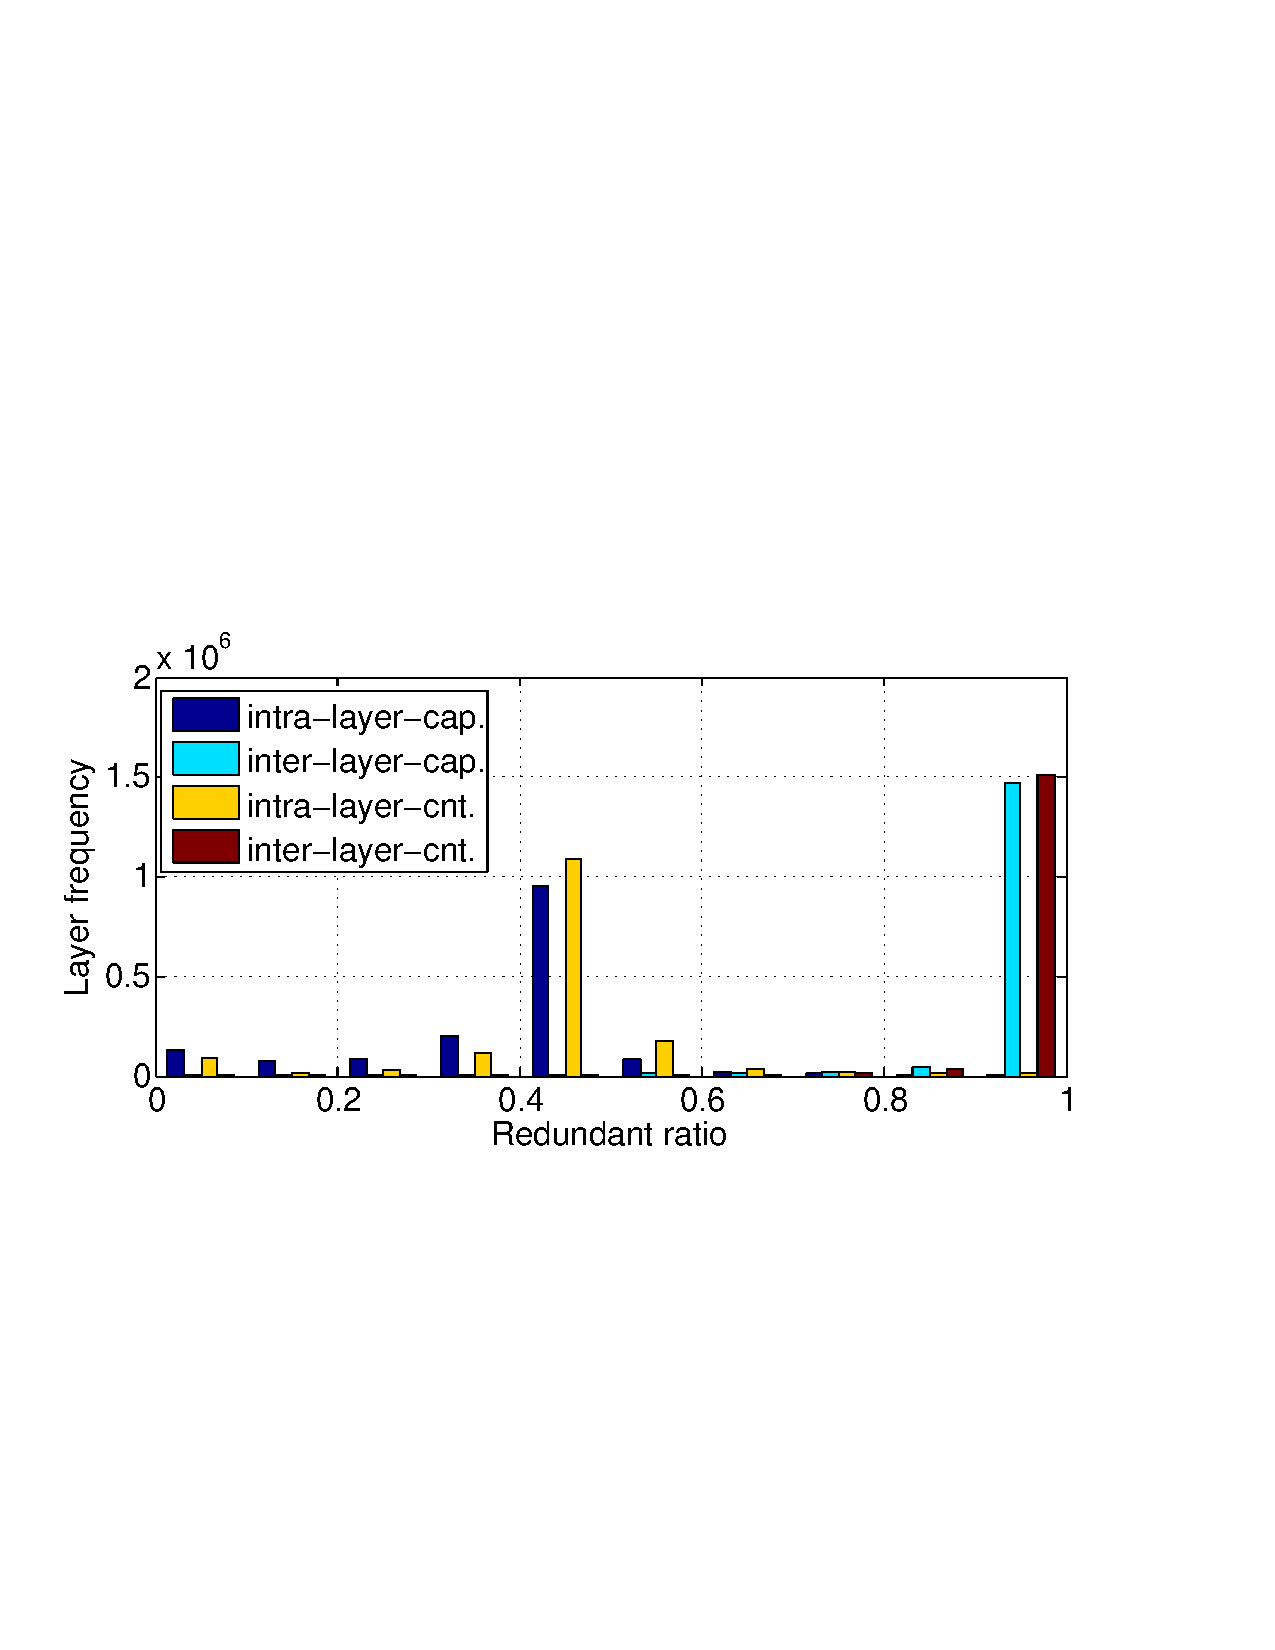
\includegraphics [width=0.4\textwidth]{graphs/layer-dup-ratio-pdf} }
%\caption{Layer redundant ratio} \label{fig:layer-dedup-ratio} \end{figure}

%\paragraph{Inter-layer redundant ratio} Inter-layer redundant ratio is shown
%in Figure~\ref{fig:layer-dedup-ratio}

%\subsection{Redundant ratio for images} \paragraph{Finding 3: Similar to
%layer, \% of images contains \% of inter-image redundant files and \% of image
%contains \% of intra-image redundant files, indicating that large amount of
%files are replicated across different images and plenty of redundant files are
%replicated within each image}

%\begin{figure} \centering \subfigure[CDF of intra/inter-image redundant ratio
%in terms of file count(denoted as *-cnt.)/capacity(denoted as
%*-cap.)]{\label{fig:image-dedup_cdf} \includegraphics
%[width=0.4\textwidth]{graphs/image-dup-ratio-pdf} } \subfigure[Histogram of
%intra/inter-image redundant ratio in terms of file count(denoted as
%*-cnt.)/capacity(denoted as *-cap.)]{\label{fig:image-dedup_hist}
%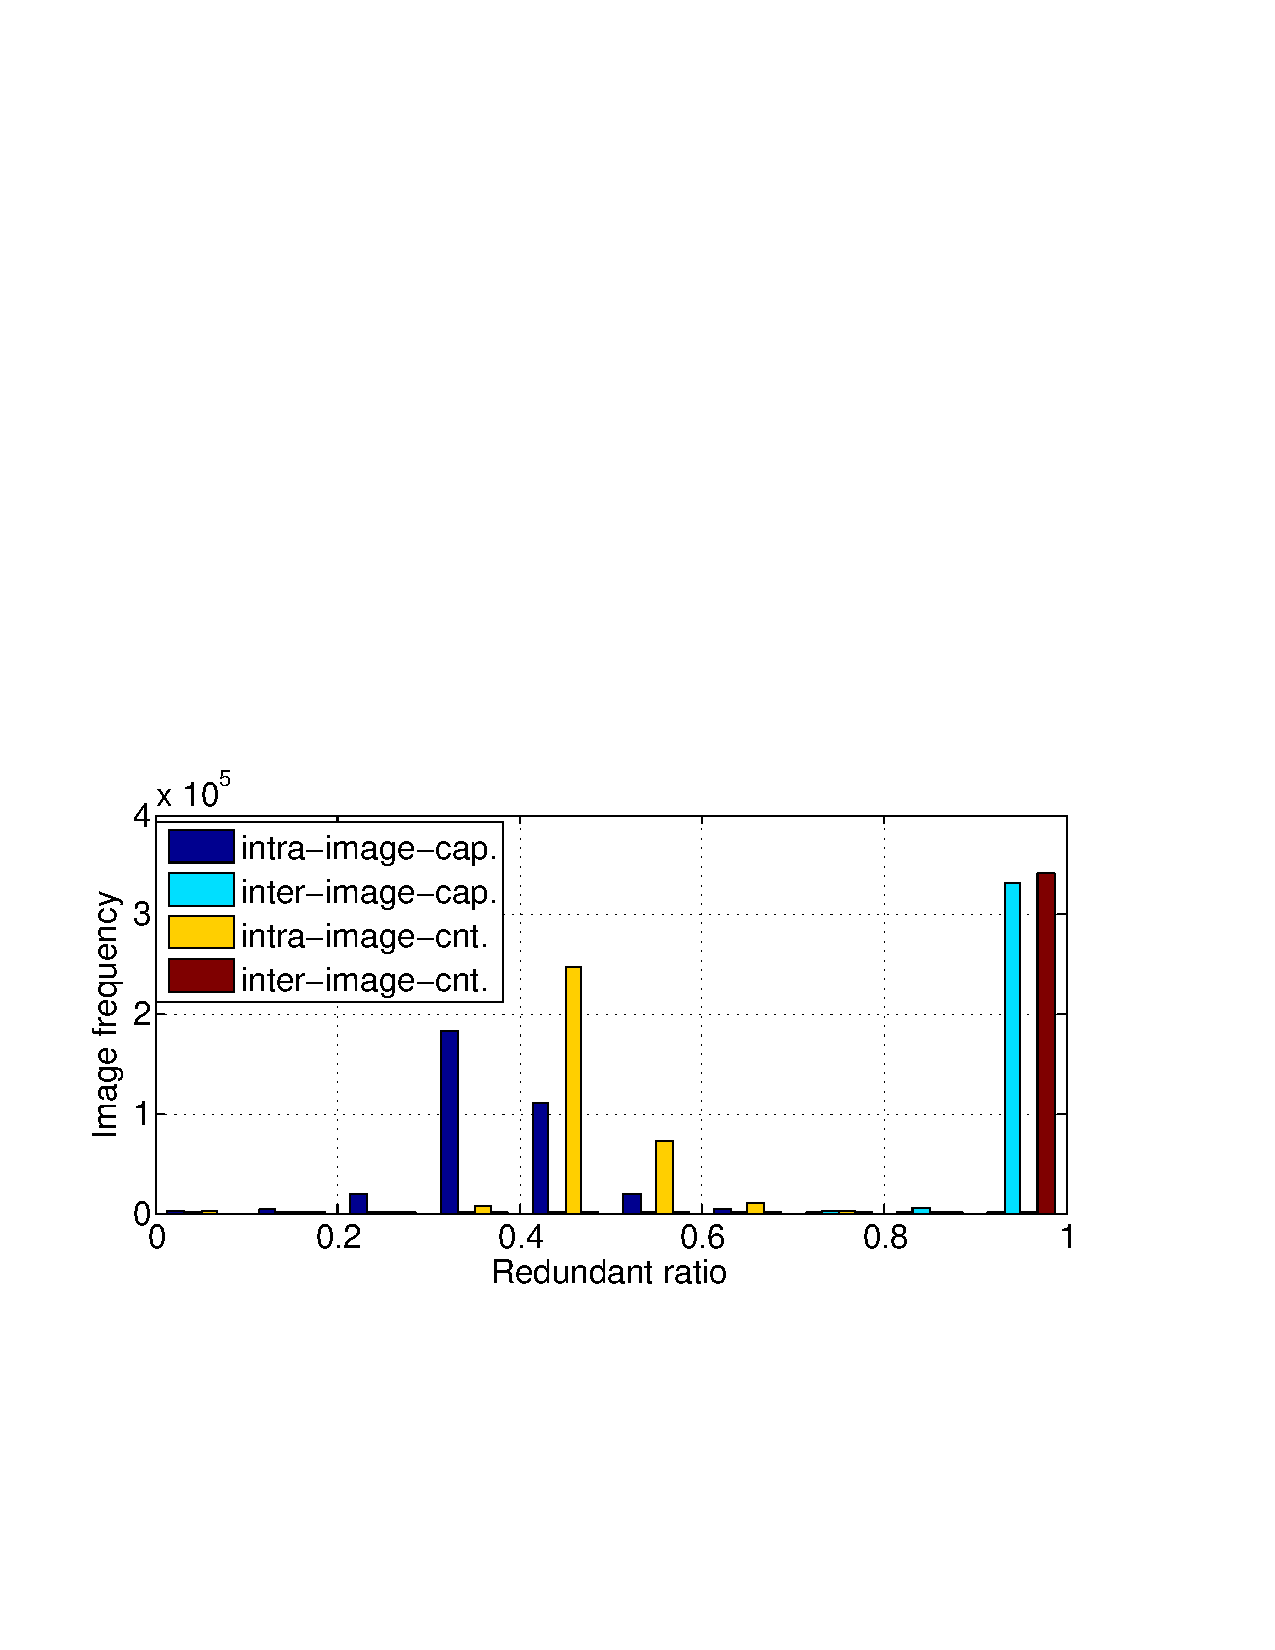
\includegraphics [width=0.4\textwidth]{graphs/image-dup-ratio-cdf} }
%\caption{Image redundant ratio} \label{fig:image-dedup-ratio} \end{figure}

%\paragraph{Intra-image redundant ratio} Intra-image redundant ratio is shown
%in Figure~\ref{fig:image-dedup-ratio}

%\paragraph{Inter-image redundant ratio} Inter-image redundant ratio is shown
%in Figure~\ref{fig:image-dedup-ratio}


%======================================= |             OLD VERSION
%| ======================================= \subsubsection{Overview of redundant
%ratio for layers} \begin{table} \centering \scriptsize
%%\begin{minipage}{.5\linewidth} \caption{Intra-layer redundant ratio for
%layers in terms of file count and capacity} \label{tbl:intra_dup_ratio_layers}
%\begin{tabular}{|l|l|l|}%p{0.14\textwidth} \hline % after \\: \hline or
%\cline{col1-col2} \cline{col3-col4} ...  % after \\: \hline or
%\cline{col1-col2} \cline{col3-col4} ...  & File count & Capacity \\ \hline
%Avg. & 49.78\% & 40.09\%\\ \hline Median & - & - \\ \hline Max. & 99.99\% &
%99.99\%\\ \hline Min.  & 0.00\%  & 0.00\%\\ \hline Stdev.  &  2.14\% &
%17.18\%\\ \hline Layer dataset after intra.-dedup (Uncompressed) & -  & -\\
%\hline Total layer dataset (Uncompressed) &  -	& -\\ \hline %\hline
%\end{tabular} \end{table}

%\begin{table} \centering \scriptsize  %\begin{minipage}{.5\linewidth}
%\caption{Inter-layer redundant ratio for layers in terms of file count and
%capacity} \label{tbl:inter_dup_ratio_layers}
%\begin{tabular}{|l|l|l|}%p{0.14\textwidth} \hline % after \\: \hline or
%\cline{col1-col2} \cline{col3-col4} ...  % after \\: \hline or
%\cline{col1-col2} \cline{col3-col4} ...  & File count & Capacity \\ \hline
%Avg. & 98.75\% & 97.33\%\\ \hline Median & - & - \\ \hline Max. & 1 & 1\\
%\hline Min.  & 0.87\%  & $<$ 0.00\%\\ \hline Stdev.  &  4.70\% & 10.49\\
%\hline Layer dataset after inter.-dedup (Uncompressed) & -  & -\\ \hline Total
%layer dataset (Uncompressed) &  -	& -\\ \hline \end{tabular} \end{table}

%\subsubsection{Redundant ratio distribution}

%\paragraph{Cumulative distribution for intra-layer redundant ratio and
%inter-layer redundant ratio in terms of file count and storage capacity}



%\paragraph{Intra-layer redundant ratio by layer size in terms of file count
%and storage capacity}

%\begin{figure} \centering
%\includegraphics[width=0.5\textwidth]{graphs/inter-dedup-by-size.eps}
%\caption{Intra-layer redundant ratio by layer size.  }
%\label{fig_redundant_overhead} \end{figure}

%\subsubsection{Inter-layer redundant overhead}

%\paragraph{Histogram of intra-layer redundant ratio and inter-layer redundant
%ratio in terms of file count and storage capacity}

%\paragraph{Inter-layer redundant ratio by layer size in terms of file count
%and storage capacity}

%\subsubsection{Overview of redundant ratio for images}

%\begin{table} \centering \scriptsize  %\begin{minipage}{.5\linewidth}
%\caption{Inter-layer redundant ratio for images in terms of file count and
%capacity} \label{tbl:intra_dup_ratio_images}
%\begin{tabular}{|l|l|l|}%p{0.14\textwidth} \hline % after \\: \hline or
%\cline{col1-col2} \cline{col3-col4} ...  % after \\: \hline or
%\cline{col1-col2} \cline{col3-col4} ...  & File count & Capacity \\ \hline
%Avg. & 98.75\% & 97.33\%\\ \hline Median & - & - \\ \hline Max. & 1 & 1\\
%\hline Min.  & 0.87\%  & $<$ 0.00\%\\ \hline Stdev.  &  4.70\% & 10.49\\
%\hline Layer dataset after share.-dedup (Uncompressed) & -  & -\\ \hline Total
%layer dataset (Uncompressed) &  -	& -\\ \hline \end{tabular} \end{table}
%
%\begin{table} \centering \scriptsize  %\begin{minipage}{.5\linewidth}
%\caption{Intra-layer redundant ratio for images in terms of file count and
%capacity} \label{tbl:inter_dup_ratio_images}
%\begin{tabular}{|l|l|l|}%p{0.14\textwidth} \hline % after \\: \hline or
%\cline{col1-col2} \cline{col3-col4} ...  % after \\: \hline or
%\cline{col1-col2} \cline{col3-col4} ...  & File count & Capacity \\ \hline
%Avg. & 98.75\% & 97.33\%\\ \hline Median & - & - \\ \hline Max. & 1 & 1\\
%\hline Min.  & 0.87\%  & $<$ 0.00\%\\ \hline Stdev.  &  4.70\% & 10.49\\
%\hline Layer dataset after share.-dedup (Uncompressed) & -  & -\\ \hline Total
%layer dataset (Uncompressed) &  -	& -\\ \hline \end{tabular} \end{table}

%\subsubsection{Redundant ratio distribution} \paragraph{Cumulative
%distribution for intra-image redundant ratio and inter-image redundant ratio
%in terms of file count and storage capacity} \paragraph{Histogram of
%intra-image redundant ratio and inter-image redundant ratio in terms of file
%count and storage capacity}

